\documentclass[a4paper,10pt,twoside]{article}
%%%%%%%%%%% Packages %%%%%%%%%%
\usepackage[margin=1in]{geometry}
\usepackage{amsmath, amssymb,mathtools}
\usepackage{fancyhdr}
\usepackage{sectsty}
\usepackage{graphicx,wrapfig}
\usepackage{enumitem}
\usepackage{float}
\usepackage{braket}
\usepackage{bbm}
\usepackage{tikz,calc}


%%%%%%%%%%% Macros %%%%%%%%%%
\def \note#1 {\paragraph{\bfseries #1}}
\def \dd {{\rm d}}
\def \id {{\mathbbm{1}}}
\def \order {\mathcal{O}}
\def\bquad{\mkern-18mu}
\DeclareMathOperator{\trace}{tr}

%%%%%%%%%%% Tikz Definitions %%%%%%%%%%
\usetikzlibrary{shapes, arrows,positioning,fit}
\tikzstyle{plain} = [draw,thick,circle,inner sep=0,minimum size=0.5cm,font=\footnotesize]
\tikzstyle{mps} = [draw,thick,circle,fill=blue!40,inner sep=0,minimum size=0.5cm]
\tikzstyle{mpo} = [draw,thick,diamond,fill=red!60,inner sep=0,minimum size=0.5cm]
\tikzstyle{blob} = [draw,thick,rectangle,rounded corners=.25cm,fill=blue!40]
\tikzstyle{index} = [-,thick,font=\footnotesize]
\tikzstyle{virtual} = [-,thick,dotted,font=\footnotesize]


\def\pair{\tikz[baseline=-0.5ex]{
\fill (0,0) circle (1.5pt) coordinate (A);
\fill (1.5ex,0) circle (1.5pt) coordinate (B);
\draw (A)--(B);}
}
%%%%%%%%%%% Formatting %%%%%%%%%%
\pagestyle{fancy}
\renewcommand{\footrulewidth}{1pt}

\fancyhf{}
\lhead{27/04/2017}
\chead{Quantum Information Methods in Many-Body Physics}
\rhead{PH2269}
\lfoot{Giacomo Giudice~~~~giacomo.giudice@mpq.mpg.de}
\rfoot{Page \thepage}

\allsectionsfont{\normalfont\sffamily}

%%%%%%%%%%% Here Begins Document %%%%%%%%%%
\begin{document}
\title{\vspace{-1cm}\sffamily Homework 2\vspace{-1cm}}
\author{}
\date{}
\maketitle
\thispagestyle{fancy}


\begin{section}{Tensor Network Diagrams}
Let us review the diagrammatic notation for tensors. 
As you may remember tensors can be represented by a circle with a number of legs, each leg corresponding to one of its indices.
The number of indices of tensor is called its {\em rank}.
A {\em contraction} between a set of tensors is the sum over all possible values of the repeated indices. 
\begin{figure}[H]
  \centerline{
    \begin{tikzpicture}[auto, node distance=1cm]
      \node (l1) {scalar};
      \node[plain,right=of l1]  (s) {};
      \node[right=of s] (l2) {vector};
      \node[plain,right=of l2]  (v) {};
      \draw[index] (v.north) -- +(0,0.5) node[left]{$i$};
      \node[right=of v] (l3) {matrix};
      \node[plain,right=of l3]  (m) {};
      \draw[index] (m.north) -- +(0,0.5) node[left]{$i$};
      \draw[index] (m.south) -- +(0,-0.5) node[left]{$j$};
      \node[right=of m,align=center] (l4) {tensor};
      \node[plain,right=of l4]  (t) {};
      \draw[index] (t.north) -- +(0,0.5) node[left]{$i$};
      \draw[index] (t.east) -- +(0.5,0) node[above]{$j$};
      \draw[index] (t.south) -- +(0,-0.5) node[right]{$k$};
      \draw[index] (t.west) -- +(-0.5,0) node[below]{$l$};
    \end{tikzpicture}
  }
\end{figure}
Draw the diagrams associated to the contractions
\begin{align*}
  {\rm (a)}~\sum_i A_i B_i\,, \qquad 
  {\rm (b)}~\sum_j A_{ij} B_{jk}\,, \qquad
  {\rm (c)}~\sum_{i,j,k,l,n} A_{ij} B_{ijkl} C_{km} D_{lnn}
\end{align*}
and  make sure to write down the indices explicitly. 
What is the rank of each resulting tensor?

Let $A$, $B$, $C$, $D$, $E$ be five square matrices. 
Draw the diagram of $\trace(ABCDE)$. 
Can you illustrate the cyclic property of the trace in this representation?
\end{section}

\begin{section}{PEPS Satisfy the Area Law --- In Three Acts}
\paragraph{Act I}
Consider a general pair of entangled systems: $\ket{\psi} = \sum_{n,m} c_{n,m} \ket{n}\ket{m}$, with $n=1,\dots,D_1$ and $m=1,\dots,D_2$.
Show that the entanglement is upper-bounded by $\log_2\min(D_1,D_2)$.
Show that this bound is still valid after acting with a local map $P = P_1 \otimes P_2$, where  $P_{1,2}: \mathbb{C}^{D_{1,2}} \to \mathbb{C}^{D_{1,2}^\prime}$.

\paragraph{Act II}
\begin{wrapfigure}{r}{6.5cm}
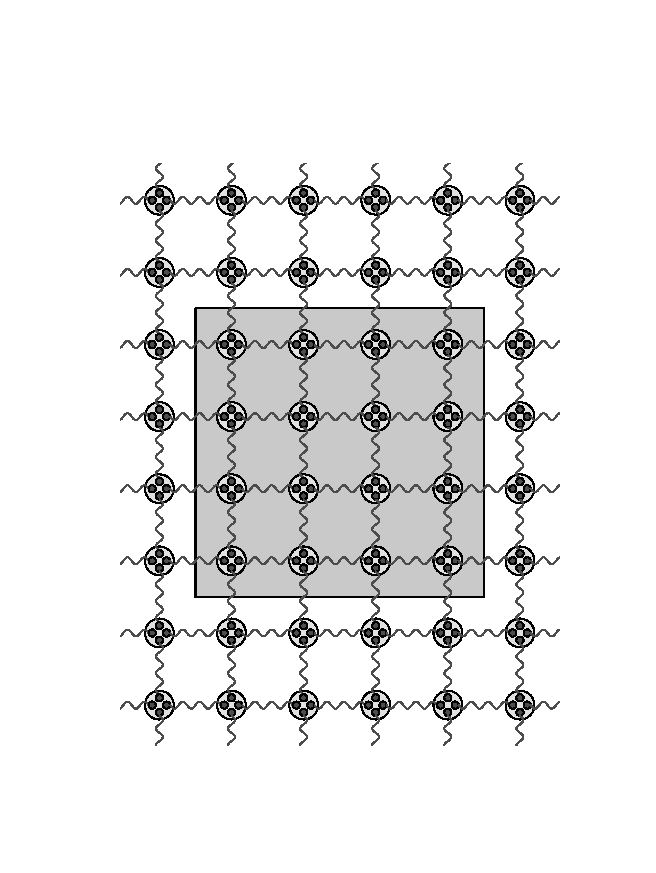
\includegraphics[width=6.5cm]{peps.pdf}
\end{wrapfigure}
Now consider a lattice, composed of $N$ nodes of coordination number $z$.
On each node we assign $z$ $D$-level systems, each entangled with a system on a neighboring node.
The total wavefunction is then $\ket{\varphi} = \ket{\pair}^{\otimes z N/2}$. 
Let $\mathcal{A}$ be an region of this lattice.
Let us now show that this construction satisfies the area law.
\begin{itemize}
  \item What is the maximum entanglement of a single pair $\ket{\pair}$?
  \item Show that the entanglement of $\mathcal{A}$ with respect to its surrounding $\bar{\mathcal{A}}$ depends only on the pairs cut by $\partial \mathcal{A}$.
%  \item What is the maximum rank of the reduced density matrix $\rho_\mathcal{A}$?
  \item Derive an upper-bound for the entanglement entropy of $\mathcal{A}$ that is an area law.
\end{itemize}

\paragraph{Act III} We now construct a \emph{Projected Entangled Pair State} (PEPS). 
We apply a map $A$: $(\mathbb{C}^D)^z \to \mathbb{C}^d$, on every node: $\ket{\rm PEPS} = A_1A_2\dots A_N \ket{\varphi}$.
Show that the entanglement of $\mathcal{A}$ still obeys an area law.
\note{Tip} If you are stuck, start by considering a $z=2$ lattice and then going to higher dimensions.
\end{section}

\begin{section}{The AKLT State}

Remember the addition of angular momentum from your quantum mechanics course?
Or did you think you could forget Clebsch--Gordon coefficients?
Convince yourself that by combining two spin-1/2 you obtain the triplet
\[
  \ket{+} = \ket{\uparrow \uparrow} , \qquad
  \ket{0} = \frac{\ket{\uparrow \downarrow} + \ket{\downarrow \uparrow}}{\sqrt{2}} , \qquad
  \ket{-} = \ket{\downarrow \downarrow} ,
\]
associated to spin-1, and the spin-0 singlet
\[
  \ket{\pair} = \frac{\ket{\uparrow \downarrow} - \ket{\downarrow \uparrow}}{\sqrt{2}} .
\]
\begin{figure}[h]
  \centerline{
\includegraphics[width=0.5\textwidth]{aklt_state.pdf}}
\end{figure}

Let us now construct a state by using $2L$ auxiliary spin-1/2 states for a chain of $L$ sites. 
In this construction
\[
  \ket{\Phi} = \sum_{\mathbf{a},\mathbf{b}} c_{\mathbf{a}\mathbf{b}} \ket{\mathbf{a},\mathbf{b}} ,
\]
where $\ket{\mathbf{a}} = \ket{a_1,\dots,a_L}$ and $\ket{\mathbf{b}} = \ket{b_1,\dots,b_L}$ represent the first and second spin-1/2 on each site.
To encode the singlet bonds between $b_i$ and $a_{i+1}$ we introduce a matrix  
\[
\Sigma=\frac{1}{\sqrt{2}}
  \begin{pmatrix}
    0 & 1\\
    -1 & 0
  \end{pmatrix}
\]
and write down the state with singlets as 
\[
  \ket{\Phi} = \sum_{\mathbf{a},\mathbf{b}} \Sigma_{b_1 a_2} \Sigma_{b_2 a_3} \dots \Sigma_{b_{L-1} a_L} \Sigma_{b_L a_1} \ket{\mathbf{a},\mathbf{b}} ,
\]
To perform the spin addition, we introduce a mapping $M$ from the state of the two auxiliary spins-1/2 $\ket{a_i}\ket{b_i} \in \{\ket{\uparrow},\ket{\downarrow}\}^{\otimes 2}$ to the states of the physical spin-1 $\ket{\sigma_i} \in \{\ket{+},\ket{0},\ket{-}\}$. 
Write the local mapping  $M^\sigma_{ab} \ket{\sigma} \bra{a, b}$ as three $ 2\times 2$ matrices, one for each $\sigma$.

The total mapping is then 
\[
  \mathcal{M} = \sum_{\boldsymbol{\sigma}} \sum_{\mathbf{a},\mathbf{b}} M^{\sigma_1}_{a_1 b_1} M^{\sigma_2}_{a_2 b_2} \dots M^{\sigma_L}_{a_L b_L} \ket{\boldsymbol{\sigma}} \bra{\mathbf{a},\mathbf{b}} 
\]
Deduce the form of the state after applying the mapping and write it as 
\[
  \ket{\Psi} = \sum_{\boldsymbol{\sigma}} \trace{\left(A^{\sigma_1} A^{\sigma_2} \dots A^{\sigma_L}\right)} \ket{\boldsymbol{\sigma}}
\]
where each $A$ is a rank-3 tensor. 
Give the explicit form of $A^\sigma$ for each $\sigma$.
Finally, draw the associated diagram.

\note{Note} Notice how the trace is used to express the periodic boundary conditions.

\end{section}

\begin{section}{Some Matrix Product States}
A \emph{Matrix Product State} (MPS) is a state describing a one-dimensional system expressed in the form
\[
  \ket{\rm MPS} = \sum_{n_1,\dots n_N} \trace{\left(A^{n_1} A^{n_2} \dots A^{n_N}\right)} \ket{n_1,\dots n_N}
\]
where each $A^{n_i}$ can be seen as a matrix for each entry $n_i$.  
More precisely  it is the decomposition of a high-rank tensor into a series of rank-3 tensors (not necessarily the same) contracted sequentially, hence the name \emph{Tensor Train decomposition}, used in mathematics and computer science.
Construct the MPS --- i.e. write down the tensors $A^{n_i}$ --- associated to the following $N$-qubit states:
\[
  {\rm (a)}~\ket{\rm Prod} = \ket{1 1 1 1 1} ,\qquad 
  {\rm (b)}~\ket{\rm GHZ} = \ket{0 0 0 0} + \ket{1 1 1 1} ,\qquad
  {\rm (c)}~\ket{\rm W} = \ket{1 0 0} + \ket{0 1 0} +  \ket{0 0 1}. 
\]
Do not worry about normalizing the states.
\note{Bonus} Construct the first two states for a two-dimensional square lattice in the thermodynamic limit.
\end{section}


\begin{section}{Multipartite Entanglement}
Let $\ket{\psi}$ be a 4-qubit state defined in terms of the Bell states
\[
  \ket{\psi} \propto \ket{\Phi^+}_{AB} \otimes \ket{\Phi^+}_{CD} +  \ket{\Psi^+}_{AB} \otimes \ket{\Psi^+}_{CD} .
\]
Normalize the state and numerically compute the entanglement of the partitions of $(A)(BCD)$, $(AB)(CD)$ and $(ABC)(D)$ by Schmidt decomposition.
\note{Tip} Test your code with states like $\ket{\Phi^+}_{AB}\ket{00}_{CD}$. Which are the entangled qubits in this case?
\end{section}

\begin{section}{Free Bosons on a Lattice}
Consider $N \in \mathbb{N}$ bosons on a one dimensional lattice of $R$ sites described by the Hamiltonian
\[
  \hat{H} = -t\sum_{j=1}^R \left( \hat{a}_j^\dag \hat{a}_{j+1} + \hat{a}_j \hat{a}_{j+1}^\dag \right)
\]
where $\hat{a}_j$  are the bosonic operators satisfying $[\hat{a}_i,\hat{a}_j^\dag] = \delta_{i,j}$, and $t > 0$. Assume periodic boundary conditions, i.e. $\hat{a}_{N+1} = \hat{a}_1$.
In momentum-space this Hamiltonian is diagonal
\[
  \hat{H} = \sum_k \epsilon_k \hat{b}_k^\dag \hat{b}_k
\]
where $\hat{b}_k = \frac{1}{\sqrt{R}} \sum_j e^{-2\pi ijk/R}\hat{a}_j$ are the Fourier-transformed annihilation operators.
Compute the dispersion relation $\epsilon_k$ --- is the system gapped?
The ground state is given by all particles at $k=0$,
\[
  \ket{\Psi_0} = \frac{1}{\sqrt{N!}} (\hat{b}_0^\dag)^N \! \ket{0}
\]
What is $\ket{\Psi_0}$ in real space?

 
We now separate the system into two parts: $A$, composed of the first $L$ sites, and $\bar{A}$, composed of $R-L$ sites.
The quantity of interest is the entanglement between $A$ sites and the rest, where $ L \ll R$.
This bipartition of the Hilbert space is achieved by defining the operators
\[
  \hat{a}_A^\dag = \frac{1}{\sqrt{L}} \sum_{j \in A} \hat{a}_j^\dag, \qquad  \hat{a}_{\bar{A}}^\dag = \frac{1}{\sqrt{R -L}} \sum_{j \in \bar{A}} \hat{a}_j^\dag .
\]
that divide the Fock space into the tensor product of the first $L$ modes with the rest.
Show that, using the binomial formula, 
\[ 
  \ket{\Psi_0} = \sum_{n=0}^N \sqrt{{N\choose n}} \left(\frac{L}{R}\right)^{\frac{n}{2}} \left(\frac{R-L}{R}\right)^{\frac{N-n}{2}} \bquad \ket{n}_A\ket{N-n}_{\bar{A}},
\]
where $\ket{n}_A = (1/\sqrt{n!}) (\hat{a}_A^\dag)^n \ket{0}$ and similarly for $\bar{A}$.
In this representation, the density operator for the first subsystem is immediate: $\hat{\rho}_A = \sum_n \rho_n \ket{n}\bra{n}$.
When $N$ is large, we can replace the sum by an integral, and show that 
\[
  \rho(n) = \frac{1}{\sqrt{2 \pi \sigma^2}} \exp{\left( -\frac{(n-n_0)^2}{2\sigma^2}\right)} .
\]
with $n_0 = NL/R$ and $\sigma = NL(R-L)/R^2$.
The entanglement entropy will then be 
\[
  E_A = - \int_{-\infty}^\infty \bquad \dd n \, \rho(n) \log \rho(n) ,
\]
Perform the integral, the leading order should be $E_A \sim \log \sigma$. 
Finally, take the limit $N,R \to \infty$ with the ratio $N/R$ fixed, and obtain 
\[
  E_A = \frac{1}{2}\log L + \order(1)
\]
Briefly comment on this result.
\end{section}
\end{document}
%%%%%%%%%%% Here Ends Document %%%%%%%%%%
